\documentclass[a4paper]{article}

\usepackage[utf8]{inputenc}
\usepackage[a4paper]{geometry}
\usepackage[english,ngerman]{babel}
\usepackage[hidelinks]{hyperref}
\usepackage{graphicx}
\usepackage{textcomp}
\usepackage{tikz}
\usepackage[scaled]{helvet}
\usepackage{titling}
\usepackage[nottoc,numbib]{tocbibind}

% remove space above title
\setlength{\droptitle}{-5em}

%symbol for external links
\newcommand{\ExternalLink}{
    \tikz[x=1.2ex, y=1.2ex, baseline=-0.05ex]{
        \begin{scope}[x=1ex, y=1ex]
            \clip (-0.1,-0.1) 
                --++ (-0, 1.2) 
                --++ (0.6, 0) 
                --++ (0, -0.6) 
                --++ (0.6, 0) 
                --++ (0, -1);
            \path[draw, 
                line width = 0.5, 
                rounded corners=0.5] 
                (0,0) rectangle (1,1);
        \end{scope}
        \path[draw, line width = 0.5] (0.5, 0.5) 
            -- (1, 1);
        \path[draw, line width = 0.5] (0.6, 1) 
            -- (1, 1) -- (1, 0.6);
    }
}

\title{WP Computergrafik\\
    \small{Abschlussprojekt Ausarbeitung} \\
    \Large{\textit{\\Simulation von Landschaftstopologien mithilfe einer fraktalen Rauschfunktion auf der Basis pseudozufälliger Gradientwerten}} \\
    \Large{\textbf{\\Ausarbeitung}}}

\author{Student: Adrian Helberg \\ \\ MatrikelNr.: 2309051 \\ \\  Prüfer: Prof. Dr. Philipp Jenke}
\date{Abgabe: \today}

\begin{document}

	\maketitle
	\pagenumbering{gobble}
	\newpage 
	\pagenumbering{arabic}
	\tableofcontents 
	\newpage 

	%%%%%%% PROJEKTSTRUKTUR %%%%%%%

	\section{Projektstruktur}

    
	%%%%%%% MOTIVATION %%%%%%%

	\section{Motivation}	

	Die Generierung von Landschaftstopologien findet zahlreiche Anwendung in der Entwicklung von Computerspielen. Um eine der Natur ähnlichen Umgebung zu simulieren, können mithilfe 		von fraktalen Rauschfunktionen Muster berechnet werden, welche in Landschaften mit natürlichen Phänomenen wie Wolken, Berge und Wasser, übersetzt werden können.\\
	Damit eine simulierte Spielwelt nicht allzu abstrakt wird und der Vorstellungskraft eines Spielenden entspricht, wird auf oben genannte Muster zurückgegriffen, um so eine Spielwelt 			zu erschaffen, welche der Natur ähnlich ist.\\
	
	%%%%%%% Ziele %%%%%%%

	\section{Ziele}

	Im Rahmen des WP Projektes \glqq Computergrafik\grqq{}  besch\"aftigt sich diese Arbeit mit einer Implementierung eines erweiterten \glqq Perlin Noice\grqq{} -Algorithmus auf der 		Basis des im gleichnamigen Praktikums zur Verfügung gestellten Kernprojektes.

	\subsection{Zielsetzung}

	Ziel dieser Arbeit ist eine Generierung simulierter, randomisierter Spielwelten, welche mit verschiedenen Farben, die repräsentativ für die Natur funktionieren (Gr\"un für Wiesen, 			Blau f\"ur Wasser, Grau f\"ur Gestein usw.), und festen Assets (B\"aume, Steine usw.) \glqq zusammengebaut\grqq{}  wird.\\
	Des weiteren werden verschiedene Geb\"aude-Assets dazu verwendet D\"orfer in der generierten Spielwelt zu gestalten und sie in geeigneter Lage zu platzieren.\\ \\
	D\"orfer sollen durch eine Straße miteinander verbunden werden.

	\newpage

	\subsection{Ergebnis}
	Eine oben genannte, generierte Spielwelt soll mit dem Vuforia\textregistered{} - Projekt auf dem Smartphone dargestellt werden können. Beispielsweise über einen Marker. \\
	Wie eine so dargestellte Spielwelt in etwa aussehen könnte, kann der Praktikumsaufgabe 4 (Aufgabenblatt 4: Kurven und Splines) entnommen werden.
	Hier sieht man eine Szene, in der Berge, Wolken und B\"aume dargestellt und farblich hervorgehoben sind. Diese Szene kann als Beispiel f\"ur eine generierte Spielwelt dieses
	Projekts betrachtet werden.\\
	Wie \"ahnlich am Ende beide Szenen sein werden, kann man hier noch nicht genauer spezifizieren. \\

	Die Position der D\"orfer wird anhand einiger Kriterien berechnet:

	\begin{itemize}
		\item Neigung des Terrains
		\begin{itemize}
			\item Das Terrain sollte m\"oglichst horizontal sein
			\item Keine D\"orfer an Bergh\"angen; Es sollen T\"aler entstehen
			\item Ein Grenzwert soll ermittelt werden, ab wann sich die Positionierung eines Dorfes nicht mehr eignet
		\end{itemize}
		\item Flussn\"ahe
		\begin{itemize}
			\item Nach Abbild der Wirklichkeit sollen D\"orfer in der N\"ahe der Ressource \glqq Wasser\grqq{} sein
		\end{itemize}
		\item Straßenanbindung
		\begin{itemize}
			\item D\"orfer sollen miteinander verbunden werden (Straßenverbindung)
			\item Die D\"orfer sollen anhand der M\"oglichkeit einer Straßenanbindung positioniert werden.
		\end{itemize}
	\end{itemize}
		
	\newpage

	%%%%%%% ALGORTIHMUS %%%%%%%

	\section{Algorithmus}
	Der folgende Pseudocode beschreibt die Implamentation des \glqq Perlin Noice\grqq{} Algorithmus.

	%%%%%%% PSEUDOCODE %%%%%%%

	\subsection{Pseudocode}

	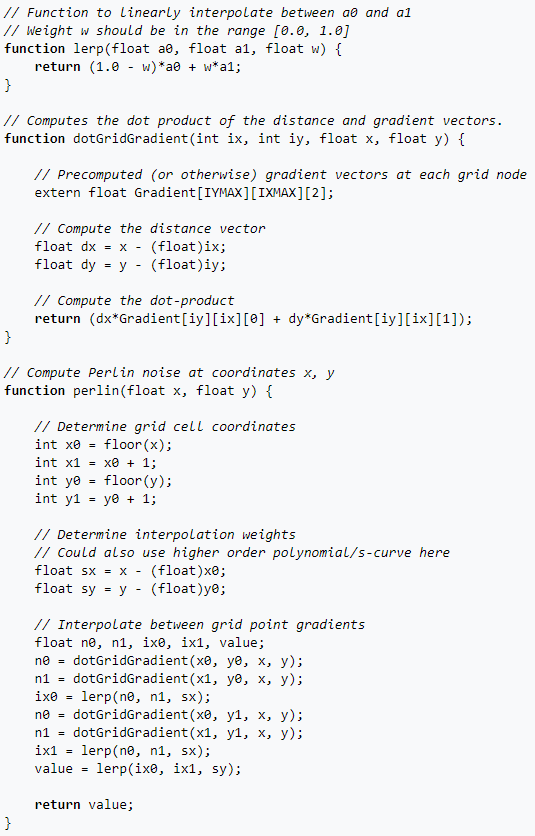
\includegraphics[height=18cm]{pseudo_code.png} \\
	Perlin Noise \url{https://en.wikipedia.org/wiki/Perlin_noise} \\


	%%%%%%% VORGEHEN %%%%%%%

	\section{Vorgehen}
		Da es nur schwer vorherzusagen ist, wie lange eine Implementation der geplanten Ziele dauert und auf welche Probleme bei der Entwicklung gestoßen wird,
		wird dieses Projekt mit dem sogenannten \glqq Prototyping \grqq{}, eine Methode der Softwareentwicklung, erarbeitet. \\
		Genauer handelt es sich um ein exploratives Prototyping, welches zur Bestimmung der Anforderungen und zur Beurteilung bestimmter Problemlösungen verwendet
		wird und sich dabei auf die Funktionalitäten des Systems konzentriert.

		%%%%%%% HERAUSFORDERUNGEN %%%%%%%

		\subsection{Herausforderung}
		Die gr\"o"ste  Herausforderung besteht hier bei dem Zusammenspiel zwischen den mathematischen Funktionen und dem Aufbauen der Spielwelt nach dessen Ergebnissen.

		%%%%%%% ZEITPLAN %%%%%%%

		\subsection{Zeitplan}
		Das Abschlussprojekt erstreckt sich \"uber folgende Meilensteine:\\

		\begin{tabular}{l | l}
  			Datum & Beschreibung \\
			\hline \\
			bis 04.02.2018 & Planung / Expos\`e \\ \\
			bis 12.03.2017 & Pr\"asentation + Abgabe \\
 		\end{tabular}

		
	%%%%%%% QUELLEN %%%%%%%

	\section{Quellen}
	
	\begin{tabular}{l l}
		Perlin Noise & \url{https://en.wikipedia.org/wiki/Perlin_noise} \\
		Understanding Perlin Noise & h\url{ttp://flafla2.github.io/2014/08/09/perlinnoise.html} \\
		The Perlin noise math FAQ & \url{https://mzucker.github.io/html/perlin-noise-math-faq.html} \\
	\end{tabular}
   
\end{document}